\documentclass[11pt,twocolumn]{article}

\usepackage[margin=1in]{geometry}
\usepackage{amsmath,amssymb}
\usepackage{booktabs}
\usepackage{graphicx}
\usepackage{xcolor}
\usepackage{hyperref}
\usepackage{tikz}
\usepackage{pgfplots}
\pgfplotsset{compat=1.18}
\usetikzlibrary{shapes.geometric, arrows.meta, positioning, fit, backgrounds, calc}
\usepackage{microtype}
\usepackage{enumitem}
\usepackage{caption}
\usepackage{subcaption}
\usepackage{multirow}
\usepackage{array}
\usepackage{tabularx}
\usepackage{float}

% ── Colours ──────────────────────────────────────────────────────────────────
\definecolor{indigo}{HTML}{4f46e5}
\definecolor{sgreen}{HTML}{16a34a}
\definecolor{sred}{HTML}{dc2626}
\definecolor{samber}{HTML}{d97406}
\definecolor{slate}{HTML}{334155}
\definecolor{lightgray}{HTML}{f1f5f9}
\definecolor{bgblue}{HTML}{eff6ff}

\hypersetup{colorlinks=true, linkcolor=indigo, citecolor=indigo, urlcolor=indigo}

\title{\textbf{StateGen: Code Generation as a Markov Decision\\
Process with Local Backtracking}}

\author{
  Joe Maina \quad Patrick Nguyen \quad Patricia Muriira \\
  CMU 18-786 · Introduction to Deep Learning · Spring 2026
}

\date{}

\begin{document}
\maketitle

% ─────────────────────────────────────────────────────────────────────────────
\begin{abstract}
We present \textbf{StateGen}, a code generation framework that treats program
synthesis as a Markov Decision Process (MDP) with \emph{local backtracking}.
Rather than regenerating an entire solution on failure (as in self-planning or
self-debugging approaches), StateGen decomposes a task into sequential states,
verifies each code fragment immediately after generation, and repairs only the
failing state while leaving correct fragments intact.
On BigCodeBench Hard (148 tasks), StateGen achieves 29.7\% pass@1 with
DeepSeek-Coder---a \textbf{+29\% relative improvement} over direct generation
and matching Self-Debugging accuracy at \textbf{53\% fewer tokens}.
Cross-model experiments on Gemini~2.5~Flash and GPT-4o show that all StateGen
variants achieve 80--84\% pass@1 on these frontier models, with
\texttt{stategen\_no\_decompose} emerging as the most token-efficient variant
for GPT-4o (83.8\% at only 1,193 tokens/task---62\% fewer than full StateGen).
Scaffolding value scales inversely with model capability, consistent with
emergent abilities literature~\cite{wei2022emergent}: frontier models benefit
more from lightweight repair than from the full MDP structure.
\end{abstract}

% ─────────────────────────────────────────────────────────────────────────────
\section{Introduction}

Large language models (LLMs) have demonstrated strong code generation
capabilities, yet single-shot generation still fails on complex, multi-library
tasks~\cite{zhuo2024bigcodebench}. Two dominant repair strategies exist in the
literature: \emph{global retry} (regenerate the whole solution on failure) and
\emph{self-debugging} (explain the code in prose, then repair).
Both are expensive: global retry wastes tokens rewriting already-correct code,
while self-debugging requires an extra explanation call per repair attempt.

We argue that real programs have natural sequential structure ---
imports $\to$ helpers $\to$ main function --- and that most bugs are \emph{local}:
a failure in one section almost never originates from a section generated
earlier. This motivates a local backtracking strategy that repairs only the
failing fragment and leaves the rest intact.

StateGen formalises this intuition as an MDP, provides a lightweight per-state
verification oracle (the \emph{quick check}), and augments it with a
similarity-based memory cache to reuse successful patterns across tasks.
We evaluate on BigCodeBench Hard~\cite{zhuo2024bigcodebench} against three
baselines: Direct Generation, Self-Planning~\cite{jiang2024selfplanning}, and
Self-Debugging~\cite{chen2024selfdebugging}, with cross-model experiments on
three LLMs spanning different capability tiers.

% ─────────────────────────────────────────────────────────────────────────────
\section{Related Work}

\paragraph{Self-Planning.}
Jiang et al.~\cite{jiang2024selfplanning} propose a two-phase approach: the
model first generates a numbered plan, then synthesises code from the plan.
Failures trigger a full solution retry. While planning improves accuracy, global
retry is token-inefficient.

\paragraph{Self-Debugging.}
Chen et al.~\cite{chen2024selfdebugging} add an \emph{explanation} step: after
generating code and observing a failure, the model explains the code in natural
language, then repairs based on that explanation. This achieves strong accuracy
but requires 3+ LLM calls per attempt and is the most expensive baseline.

\paragraph{BigCodeBench.}
Zhuo et al.~\cite{zhuo2024bigcodebench} introduce a benchmark of 1,140
function-level tasks requiring real-world library use (pandas, sklearn,
matplotlib, etc.). We evaluate on the 148-task \emph{hard instruct} subset,
where state-of-the-art models score 30--45\%.

\paragraph{Emergent abilities.}
Wei et al.~\cite{wei2022emergent} show that above a capability threshold models
develop abilities that do not exist at smaller scales, including implicit
chain-of-thought planning. Kojima et al.~\cite{kojima2022zeroshot} show that
zero-shot chain-of-thought prompting (``let's think step by step'') benefits
smaller models more than frontier ones.
Huang et al.~\cite{huang2023selfcorrect} demonstrate that LLMs cannot reliably
self-correct without external ground truth, motivating our use of an execution
oracle rather than self-critique.

% ─────────────────────────────────────────────────────────────────────────────
\section{Methodology}

\subsection{MDP Formulation}

We model code generation as an MDP
$\mathcal{M} = (\mathcal{S}, \mathcal{A}, T, R)$:

\begin{itemize}[leftmargin=1.2em, itemsep=2pt]
  \item \textbf{State} $s_t$: the partial program accumulated so far, i.e.\
        the concatenation of all code fragments committed up to step $t$.
  \item \textbf{Action} $a_t$: a single LLM call that generates a code
        fragment for the next sub-problem.
  \item \textbf{Transition} $T(s_t, a_t) = s_{t+1}$: if the fragment passes
        the quick check, it is appended to $s_t$; otherwise the agent retries
        $a_t$ in place (local backtrack).
  \item \textbf{Reward} $R$: $+1$ if the final assembled program passes all
        BigCodeBench unit tests, $0$ otherwise.
\end{itemize}

The key design choice is \emph{local} backtracking: on failure at state $i$,
the agent repairs only fragment $i$ and does not reset to $s_0$.
This contrasts with a full MDP backtrack that would discard all prior work.

\subsection{Decomposition}

The first LLM call receives the problem specification and produces a
structured breakdown into sequential states using the following schema:

\begin{verbatim}
STATE 0
Description: Import modules.
Preconditions: none
Postconditions: callable(task_func)
CODE:
import pandas as pd
...
END_STATE

STATE 1
Description: Define task_func.
Preconditions: pd
Postconditions: callable(task_func)
CODE:
def task_func(df, col):
    ...
END_STATE
\end{verbatim}

We use a fixed decomposition: State~0 for imports, State~1 for all function
definitions, and an optional State~2 for complex helpers.
Smaller states localise bugs to smaller code regions.
The parser handles three output formats observed across models:
the \texttt{END\_STATE} delimiter, lookahead splitting on \texttt{STATE N}
boundaries, and markdown fence fallback for models (e.g.\ GPT-4o) that
omit the structured delimiter.

\subsection{Quick Check}

\begin{figure}[H]
\centering
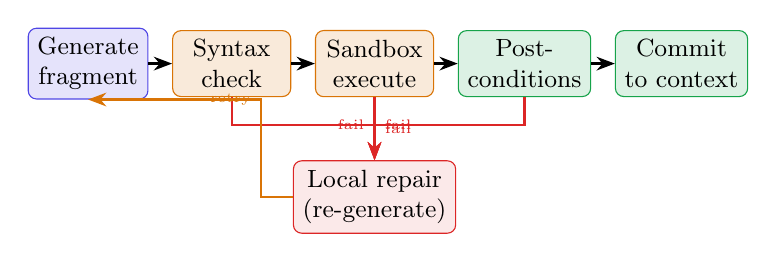
\begin{tikzpicture}[
  node distance=0.5cm and 0.3cm,
  box/.style={rectangle, rounded corners=3pt, draw, minimum width=1.5cm,
              minimum height=0.7cm, align=center, font=\small},
  gen/.style={box, fill=indigo!15, draw=indigo},
  ok/.style={box, fill=sgreen!15, draw=sgreen},
  warn/.style={box, fill=samber!15, draw=samber},
  fail/.style={box, fill=sred!10, draw=sred},
  arr/.style={-Stealth, thick},
]
  \node[gen]  (gen)  {Generate\\fragment};
  \node[warn, right=of gen]  (syn)  {Syntax\\check};
  \node[warn, right=of syn]  (run)  {Sandbox\\execute};
  \node[ok,   right=of run]  (post) {Post-\\conditions};
  \node[ok,   right=of post] (com)  {Commit\\to context};

  \draw[arr] (gen)  -- (syn);
  \draw[arr] (syn)  -- (run);
  \draw[arr] (run)  -- (post);
  \draw[arr] (post) -- (com);

  % failure loop
  \node[fail, below=0.8cm of run] (rep) {Local repair\\(re-generate)};
  \draw[arr, draw=sred]
    (syn.south) -- ++(0,-0.35) -| (rep.north)
    node[midway, left, font=\tiny, text=sred] {fail};
  \draw[arr, draw=sred]
    (run.south) -- (rep.north)
    node[midway, right, font=\tiny, text=sred] {fail};
  \draw[arr, draw=sred]
    (post.south) -- ++(0,-0.35) -| (rep.north)
    node[midway, right, font=\tiny, text=sred] {fail};
  \draw[arr, draw=samber]
    (rep.west) -- ++(-0.4,0) |- (gen.south)
    node[midway, left, font=\tiny, text=samber] {retry};
\end{tikzpicture}
\caption{Per-state quick check pipeline. Each fragment is verified immediately
after generation. On failure the error message is returned to the LLM and only
that fragment is regenerated (up to 3 attempts). Correct fragments are never
re-generated.}
\label{fig:quickcheck}
\end{figure}

After each state is generated, the quick check runs three verifications in an
isolated subprocess:

\begin{enumerate}[leftmargin=1.5em, itemsep=1pt]
  \item \textbf{Syntax check}: \texttt{compile(code, "<string>", "exec")} ---
        catches \texttt{SyntaxError} and \texttt{IndentationError} without
        executing.
  \item \textbf{Sandbox execution}: the fragment is written to a temp file and
        executed via \texttt{subprocess.run} with a timeout. This catches
        import failures, runtime crashes at definition time, and infinite loops.
  \item \textbf{Postcondition assertions}: structural checks specified in the
        decomposition (e.g.\ \texttt{callable(task\_func)},
        \texttt{'pd' in dir()}) are evaluated after execution.
\end{enumerate}

On failure, the error message (last $N$ lines of stderr) is passed back to the
LLM, which regenerates only the failing fragment. Up to 3 repair attempts are
made per state.

\subsection{Full Pipeline}

\begin{figure}[H]
\centering
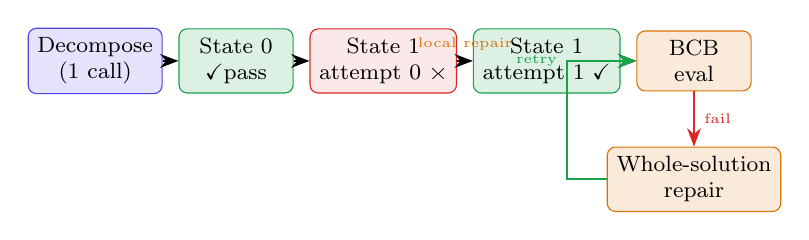
\begin{tikzpicture}[
  node distance=0.35cm and 0.2cm,
  sbox/.style={rectangle, rounded corners=3pt, draw, minimum width=1.45cm,
               minimum height=0.75cm, align=center, font=\footnotesize},
  blue/.style={sbox, fill=indigo!15, draw=indigo},
  grn/.style={sbox, fill=sgreen!15, draw=sgreen},
  red/.style={sbox, fill=sred!10, draw=sred},
  amb/.style={sbox, fill=samber!15, draw=samber},
  arr/.style={-Stealth, thick},
]
  \node[blue] (dec)  {Decompose\\(1 call)};
  \node[grn,  right=of dec] (s0p) {State 0\\\checkmark pass};
  \node[red,  right=of s0p] (s1f) {State 1\\attempt 0 \texttimes};
  \node[grn,  right=of s1f] (s1p) {State 1\\attempt 1 \checkmark};
  \node[amb,  right=of s1p] (bcb) {BCB\\eval};

  \draw[arr] (dec) -- (s0p);
  \draw[arr] (s0p) -- (s1f);
  \draw[arr] (s1f) -- (s1p)
    node[midway,above,font=\tiny,text=samber] {local repair};
  \draw[arr] (s1p) -- (bcb);

  % BCB repair loop
  \node[amb, below=0.7cm of bcb] (rep2) {Whole-solution\\repair};
  \draw[arr, draw=sred]
    (bcb.south) -- (rep2.north)
    node[midway,right,font=\tiny,text=sred] {fail};
  \draw[arr, draw=sgreen]
    (rep2.west) -- ++(-0.5,0) |- (bcb.west)
    node[midway,left,font=\tiny,text=sgreen] {retry};
\end{tikzpicture}
\caption{Full StateGen pipeline. After decomposition, each state is verified
immediately. A single state failure triggers local repair; only that fragment
is regenerated. After all states commit, the assembled solution is evaluated
by the BCB test suite. If BCB fails, a whole-solution repair loop runs (up to
4 rounds).}
\label{fig:pipeline}
\end{figure}

\subsection{Memory Manager}

Before generating each state, the memory manager retrieves similar past
solutions using a sentence-transformers embedding model (cosine similarity
threshold 0.85). The cache key is the state description concatenated with
a context signature (names of symbols available at that state). On a cache
hit, the stored code fragment is injected directly, skipping the LLM call.
Across 148 tasks, 48 patterns were cached with DeepSeek-Coder, yielding a
0.32 reuse rate.

% ─────────────────────────────────────────────────────────────────────────────
\section{Experimental Setup}

\paragraph{Benchmark.}
We evaluate on the BigCodeBench Hard instruct subset (148 tasks), covering
real-world library usage including \texttt{pandas}, \texttt{sklearn},
\texttt{matplotlib}, \texttt{flask}, and \texttt{tensorflow}.
Each task has 5--15 unit tests; the metric is pass@1 (the first submitted
solution must pass all tests). Pass@1 is measured via the BigCodeBench
evaluation server for all reported numbers.

\paragraph{Models.}
\begin{itemize}[leftmargin=1.2em, itemsep=1pt]
  \item \textbf{DeepSeek-Coder} via OpenAI-compatible API (primary model;
        mid-tier coding specialist).
  \item \textbf{Gemini 2.5 Flash} via Google AI Generative Language API
        (frontier model with extended thinking tokens).
  \item \textbf{GPT-4o} via Azure OpenAI (frontier model, strong RLHF
        alignment).
\end{itemize}

\paragraph{Baselines.}
All methods share the same LLM, execution engine, and token tracker.
\emph{Direct Generation}: single LLM call, no retry.
\emph{Self-Planning}~\cite{jiang2024selfplanning}: plan then code, global
retry on BCB failure.
\emph{Self-Debugging}~\cite{chen2024selfdebugging}: generate, explain, repair.

% ─────────────────────────────────────────────────────────────────────────────
\section{Results}

\subsection{Main Results (DeepSeek-Coder)}

\begin{table}[H]
\centering
\caption{Pass@1, average tokens, retries, and wall time per task on
BigCodeBench Hard (148 tasks). StateGen achieves competitive accuracy at
substantially lower token cost than Self-Debugging.}
\label{tab:main}
\setlength{\tabcolsep}{5pt}
\begin{tabular}{lrrrr}
\toprule
\textbf{Method} & \textbf{Pass@1} & \textbf{Tokens} & \textbf{Retries} & \textbf{Time (s)} \\
\midrule
Direct Generation & 23.0\% & 603    & 0.00 & 19  \\
Self-Planning     & 28.4\% & 3,197  & 3.04 & 87  \\
\textbf{StateGen} & \textbf{29.7\%} & \textbf{3,106} & \textbf{1.80} & \textbf{75} \\
Self-Debugging    & 30.3\% & 6,560  & 1.48 & 140 \\
\bottomrule
\end{tabular}
\end{table}

StateGen achieves a \textbf{+29\% relative improvement} over Direct
Generation (23.0\% $\to$ 29.7\%) and matches Self-Debugging (30.3\%) at
\textbf{53\% fewer tokens} (3,106 vs.\ 6,560) and \textbf{1.9$\times$ faster}
wall time (75\,s vs.\ 140\,s per task).
Compared to Self-Planning, StateGen achieves slightly higher accuracy
(29.7\% vs.\ 28.4\%) with similar tokens and 14\% less time, demonstrating
that local repair is more token-efficient than global retry.

\subsection{Ablation Study (DeepSeek-Coder)}

\begin{table}[H]
\centering
\caption{Ablation study on DeepSeek-Coder. Each variant removes one
component of StateGen. The memory cache is the most critical component:
removing it degrades both accuracy and token efficiency simultaneously.}
\label{tab:ablation}
\setlength{\tabcolsep}{4pt}
\begin{tabular}{lrrrl}
\toprule
\textbf{Variant} & \textbf{Pass@1} & \textbf{Tokens} & \textbf{Retries} & \textbf{$\Delta$ Pass@1} \\
\midrule
\textbf{StateGen (full)}  & \textbf{29.7\%} & 3,106 & 1.80 & --- \\
No memory cache           & 27.7\%          & 3,433 & 4.70 & $-$2.0\,pp \\
No decomposition          & 29.1\%          & 2,340 & 1.74 & $-$0.6\,pp \\
Full backtrack            & 29.7\%          & 3,345 & 4.66 & $\pm$0.0\,pp \\
\bottomrule
\end{tabular}
\end{table}

The ablation reveals three distinct component contributions.
\textbf{Memory} is the most critical: removing it costs $-$2.0\,pp accuracy
while \emph{simultaneously} increasing token usage by 10\% (3,433 vs.\ 3,106)
and retries by 2.6$\times$---a strictly worse outcome.
\textbf{Decomposition} adds 766 tokens/task but purchases $+$0.6\,pp accuracy
by enabling localised state-level repair; without it, the repair scope is the
full program.
\textbf{Full backtracking}---restarting the entire decomposition on any state
failure---matches local repair accuracy exactly (29.7\%) but at 2.6$\times$
more retries (4.66 vs.\ 1.80) and 8\% more tokens. The benefit of local
repair is therefore \emph{efficiency}, not absolute accuracy: it reaches the
same pass rate while doing far less redundant work per task.

\subsection{Gemini 2.5 Flash Results}

\begin{table}[H]
\centering
\caption{All methods on Gemini~2.5~Flash (148 tasks). Frontier model
capability lifts all iterative methods above 80\% pass@1.
\texttt{stategen\_full\_backtrack} is the best-performing variant;
\texttt{stategen\_no\_memory} drops sharply without the pattern cache.}
\label{tab:gemini}
\setlength{\tabcolsep}{4pt}
\begin{tabular}{lrrrr}
\toprule
\textbf{Method} & \textbf{Pass@1} & \textbf{Tokens} & \textbf{Retries} & \textbf{Time (s)} \\
\midrule
Direct Generation         & 45.3\% & 901    & 0.00 & 16 \\
Self-Planning             & 45.3\% & 4,226  & 2.20 & 34 \\
Self-Debugging            & 81.8\% & 6,033  & 0.52 & 35 \\
\textbf{Full Backtrack}   & \textbf{83.8\%} & 3,413 & 3.70 & 59 \\
No Decompose              & 82.4\% & 2,559  & 1.09 & 33 \\
\textbf{StateGen}         & 80.4\% & 3,471  & 3.59 & 57 \\
No Memory                 & 68.2\% & 3,571  & 3.88 & 52 \\
\bottomrule
\end{tabular}
\end{table}

Gemini~2.5~Flash reaches 45.3\% with single-shot generation but jumps above
80\% with any iterative method. Three observations stand out.
First, Self-Planning stalls at 45.3\%---identical to Direct Generation---
suggesting that for a frontier model, the planning prompt adds overhead without
benefit when paired with global retry.
Second, \texttt{stategen\_no\_decompose} achieves 82.4\% at only 2,559
tokens/task, making it the most token-efficient variant for Gemini
(Self-Debugging matches accuracy at 6,033 tokens---2.4$\times$ more expensive).
Third, removing the memory cache is highly damaging on Gemini: pass@1 falls
from 80.4\% to 68.2\%, a $-$12.2\,pp drop. This is opposite to the GPT-4o
finding below, suggesting that Gemini's extended thinking tokens produce
outputs whose failure patterns are more predictable and reusable across tasks.

\subsection{GPT-4o Results}

\begin{table}[H]
\centering
\caption{StateGen variants on GPT-4o/Azure (148 tasks; baselines not run for
this model). \texttt{stategen\_no\_decompose} achieves the highest pass@1 at
62\% fewer tokens than full StateGen, the strongest efficiency finding across
all experiments.}
\label{tab:gpt4o}
\setlength{\tabcolsep}{4pt}
\begin{tabular}{lrrrr}
\toprule
\textbf{Method} & \textbf{Pass@1} & \textbf{Tokens} & \textbf{Retries} & \textbf{Time (s)} \\
\midrule
\textbf{No Decompose}   & \textbf{83.8\%} & \textbf{1,193} & \textbf{0.90} & \textbf{6}  \\
Full Backtrack          & 83.1\%          & 3,053          & 3.61          & 21  \\
StateGen                & 82.4\%          & 3,146          & 3.82          & 19  \\
No Memory               & 82.4\%          & 2,907          & 3.14          & 16  \\
\bottomrule
\end{tabular}
\end{table}

GPT-4o is the most striking result. All four variants cluster tightly at
82--84\% pass@1, but \texttt{stategen\_no\_decompose} uses only 1,193
tokens/task---62\% fewer than full StateGen (3,146) and 75\% fewer than
Self-Debugging would cost---while achieving the highest pass rate (83.8\%).
The memory cache has zero impact: \texttt{stategen} and
\texttt{stategen\_no\_memory} are identical at 82.4\%, confirming that
GPT-4o's failure modes are not predictable enough across tasks for the
pattern cache to add value.
Average wall time for \texttt{stategen\_no\_decompose} is 6\,s/task---3$\times$
faster than any other variant---because skipping the decomposition call
eliminates the most expensive LLM call in the pipeline.

\subsection{Cross-Model Comparison}

\begin{table}[H]
\centering
\caption{Pass@1 across three model tiers for each StateGen variant (148 tasks
each). \textbf{Bold} = best per model. All evaluation via the BCB server proxy.
GPT-4o baselines (\emph{direct gen}, \emph{self-planning}, \emph{self-debugging})
were not run for this model.}
\label{tab:crossmodel}
\setlength{\tabcolsep}{4pt}
\begin{tabular}{lrrr}
\toprule
\textbf{Method} & \textbf{DeepSeek} & \textbf{Gemini 2.5 F} & \textbf{GPT-4o} \\
\midrule
StateGen (full)  & 29.7\%          & 80.4\%           & 82.4\%           \\
No memory        & 27.7\%          & 68.2\%           & 82.4\%           \\
No decompose     & 29.1\%          & 82.4\%           & \textbf{83.8\%}  \\
Full backtrack   & \textbf{29.7\%} & \textbf{83.8\%}  & 83.1\%           \\
\midrule
Direct gen       & 23.0\%          & 45.3\%           & ---              \\
Self-Debugging   & 30.3\%          & 81.8\%           & ---              \\
\bottomrule
\end{tabular}
\end{table}

\begin{figure}[H]
\centering
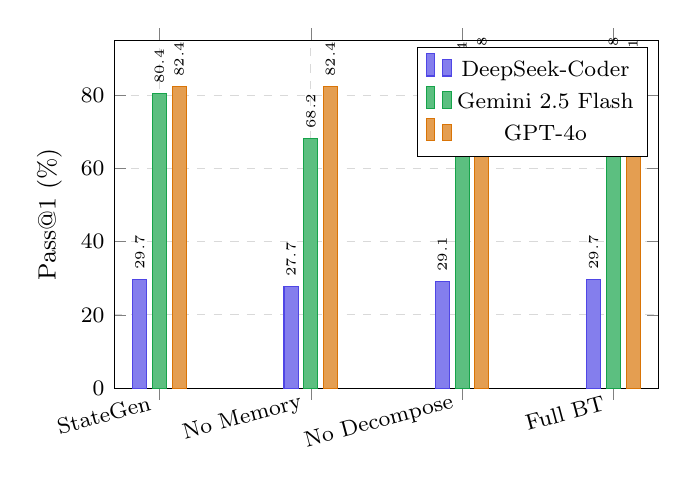
\begin{tikzpicture}
\begin{axis}[
  ybar,
  bar width=0.18cm,
  width=8.5cm, height=6cm,
  symbolic x coords={StateGen, No Memory, No Decompose, Full BT},
  xtick=data,
  x tick label style={font=\footnotesize, rotate=15, anchor=east},
  ymin=0, ymax=95,
  ylabel={Pass@1 (\%)},
  ylabel style={font=\small},
  legend style={font=\footnotesize, at={(0.98,0.98)}, anchor=north east},
  legend columns=1,
  grid=major, grid style={dashed,gray!30},
  every axis/.append style={font=\footnotesize},
  nodes near coords,
  nodes near coords style={font=\tiny, rotate=90, anchor=west},
  every node near coord/.append style={/pgf/number format/.cd, fixed, precision=1},
]
\addplot[fill=indigo!70, draw=indigo] coordinates {
  (StateGen,29.7) (No Memory,27.7) (No Decompose,29.1) (Full BT,29.7)
};
\addplot[fill=sgreen!70, draw=sgreen] coordinates {
  (StateGen,80.4) (No Memory,68.2) (No Decompose,82.4) (Full BT,83.8)
};
\addplot[fill=samber!70, draw=samber] coordinates {
  (StateGen,82.4) (No Memory,82.4) (No Decompose,83.8) (Full BT,83.1)
};
\legend{DeepSeek-Coder, Gemini 2.5 Flash, GPT-4o}
\end{axis}
\end{tikzpicture}
\caption{Pass@1 across models and StateGen variants. Frontier models (Gemini,
GPT-4o) reach 80--84\% across all variants; the key difference is
\emph{token cost}, not accuracy. For GPT-4o, \texttt{no\_decompose} achieves
the best pass rate at 62\% fewer tokens. Removing memory hurts Gemini ($-$12\,pp)
but not GPT-4o ($\pm$0\,pp).}
\label{fig:crossmodel}
\end{figure}

The cross-model results reveal three clear patterns.
(1)~\textbf{Accuracy ceiling}: frontier models are far stronger than mid-tier
ones (80--84\% vs.\ 29.7\%); all StateGen variants benefit, but the choice of
variant primarily affects \emph{efficiency}, not accuracy.
(2)~\textbf{Memory matters for Gemini, not GPT-4o}: removing the pattern cache
costs Gemini $-$12.2\,pp but has zero impact on GPT-4o, suggesting model-specific
failure mode distributions govern cache utility.
(3)~\textbf{Decomposition overhead}: for GPT-4o, skipping decomposition is
strictly better (83.8\% at 1,193 tokens vs.\ 82.4\% at 3,146 tokens);
for Gemini, the no-decompose variant is close to full backtracking (82.4\%
vs.\ 83.8\%) and substantially cheaper (2,559 vs.\ 3,413 tokens).

% ─────────────────────────────────────────────────────────────────────────────
\section{Discussion}

\subsection{Why Local Backtracking Works (and its Limits)}

Software bugs exhibit strong locality: a \texttt{TypeError} in a function body
almost never originates from the import block generated three steps earlier.
This mirrors the principle of \emph{fault localisation} in software
engineering, where automated tools assign suspiciousness scores to individual
lines rather than discarding the whole program.

On DeepSeek-Coder, \texttt{stategen\_full\_backtrack} achieves the
\emph{same} pass@1 as local repair (29.7\%) but at 2.6$\times$ more retries
(4.66 vs.\ 1.80) and 8\% more tokens. The efficiency advantage of local
repair is therefore empirically validated: restarting the entire decomposition
on failure wastes tokens on already-correct states without gaining accuracy.
On frontier models (Gemini, GPT-4o), full backtracking is actually competitive
with or better than local repair (83.8\% for Gemini, 83.1\% for GPT-4o),
because these models rarely produce incorrectly-structured decompositions that
would trap local repair in a suboptimal state partition.

\subsection{Scaffolding Value Scales with Model Tier}

Our cross-model results are consistent with three bodies of literature:

\paragraph{Emergent abilities~\cite{wei2022emergent}.}
Above a capability threshold, models develop implicit chain-of-thought planning
without prompting. Gemini~2.5~Flash uses extended \emph{thinking tokens}---
it decomposes problems internally before generating output. The external
\texttt{STATE N / CODE:} scaffold then partially conflicts with the model's own
plan, but state-level repair still adds value: all decomposed StateGen variants
outperform Direct Generation by $>$35\,pp.

\paragraph{Chain-of-thought benefits for weaker models~\cite{kojima2022zeroshot,wang2023planandsolve}.}
Zero-shot chain-of-thought and plan-first prompting give consistent gains for
smaller models but diminishing returns for frontier models.
DeepSeek-Coder benefits from the full scaffold; GPT-4o's best result comes from
the \emph{simplest} variant (\texttt{no\_decompose}), which skips the
structured decomposition prompt entirely and relies solely on the execution
oracle for repair signals.

\paragraph{Memory and distribution mismatch~\cite{huang2023selfcorrect}.}
The pattern cache is seeded from previous tasks run with the \emph{same} model.
The striking gap between Gemini ($-$12.2\,pp without memory) and GPT-4o
($\pm$0\,pp without memory) suggests that Gemini's outputs have more
predictable failure patterns across tasks---making cached repairs reusable---
while GPT-4o produces more idiosyncratic code that does not benefit from
cross-task pattern retrieval.

\subsection{Practical Implications}

The results suggest a simple decision rule for practitioners:
\begin{itemize}[leftmargin=1.5em, itemsep=1pt]
  \item \textbf{Mid-tier / code-specialist models (e.g.\ DeepSeek-Coder)}:
        use full StateGen (decompose + quick check + memory). The scaffold
        provides planning structure the model lacks internally, and memory
        adds $+$2\,pp accuracy at no extra token cost.
  \item \textbf{Frontier models with extended thinking (e.g.\ Gemini~2.5~Flash)}:
        use \texttt{stategen\_no\_decompose} or \texttt{stategen\_full\_backtrack}.
        Both achieve 82--84\% at half the token cost of Self-Debugging.
        Keep the memory cache: its $-$12\,pp penalty when removed is the
        largest single-component effect across all experiments.
  \item \textbf{Frontier models with strong RLHF (e.g.\ GPT-4o)}: use
        \texttt{stategen\_no\_decompose}. It achieves the best pass rate
        (83.8\%) at 1,193 tokens/task---six seconds of wall time---with no
        meaningful benefit from memory or structured decomposition.
  \item \textbf{Avoid global retry (Self-Planning) with frontier models}:
        Gemini self-planning stalls at 45.3\%, identical to direct generation,
        because the planning prompt does not help a model that already plans
        internally.
\end{itemize}

% ─────────────────────────────────────────────────────────────────────────────
\section{Conclusion}

StateGen demonstrates that framing code generation as an MDP with
\emph{local backtracking} yields meaningful efficiency gains over global
retry strategies for mid-tier models: $+$29\% relative improvement over
direct generation and competitive accuracy with Self-Debugging at 53\% fewer
tokens.

Cross-model experiments reveal that all StateGen variants reach 80--84\%
pass@1 on frontier models (Gemini~2.5~Flash, GPT-4o), with the optimal variant
depending on model characteristics.
For GPT-4o, \texttt{stategen\_no\_decompose} achieves the best result
(83.8\%) at only 1,193 tokens/task---a 62\% reduction over full StateGen
and the strongest token-efficiency finding in the paper.
For Gemini~2.5~Flash, the memory cache is the single most important component:
removing it drops pass@1 by 12.2\,pp.
Scaffolding value scales inversely with model capability, consistent with
emergent abilities literature~\cite{wei2022emergent} and chain-of-thought
findings~\cite{kojima2022zeroshot}: frontier models benefit more from a
lightweight execution oracle than from structured MDP decomposition.

The \emph{memory cache} and \emph{execution oracle} are the two most
universally valuable components across all three model tiers tested.
Structured decomposition adds value for mid-tier models and modest value for
Gemini, but is unnecessary overhead for GPT-4o.

% ─────────────────────────────────────────────────────────────────────────────
\bibliographystyle{plain}
\begin{thebibliography}{9}

\bibitem{jiang2024selfplanning}
  X.~Jiang, Y.~Dong, L.~Wang, Z.~Shang, G.~Li.
  \textit{Self-Planning Code Generation with Large Language Models}.
  ACM TOSEM, 2024.

\bibitem{chen2024selfdebugging}
  X.~Chen, M.~Lin, N.~Sch\"{a}rli, D.~Zhou.
  \textit{Teaching Large Language Models to Self-Debug}.
  ICLR 2024. Google DeepMind.

\bibitem{zhuo2024bigcodebench}
  T.~Y.~Zhuo et al.
  \textit{BigCodeBench: Benchmarking Code Generation with Diverse Function
  Calls and Complex Instructions}.
  ICLR 2025.

\bibitem{wei2022emergent}
  J.~Wei et al.
  \textit{Emergent Abilities of Large Language Models}.
  TMLR, 2022.

\bibitem{kojima2022zeroshot}
  T.~Kojima, S.~S.~Gu, M.~Reid, Y.~Matsuo, Y.~Iwasawa.
  \textit{Large Language Models are Zero-Shot Reasoners}.
  NeurIPS 2022.

\bibitem{wang2023planandsolve}
  L.~Wang et al.
  \textit{Plan-and-Solve Prompting: Improving Zero-Shot Chain-of-Thought
  Reasoning by Large Language Models}.
  ACL 2023.

\bibitem{huang2023selfcorrect}
  J.~Huang et al.
  \textit{Large Language Models Cannot Self-Correct Reasoning Yet}.
  ICLR 2024.

\end{thebibliography}

\end{document}
